\newpage
\section{Реконструкция края}
В данном разделе рассматривается реконструкция края (аналогично \cite{Wang2017}) 
в модели сильной связи \eqref{BHZ} из \cite{Bernevig2006}.

Как известно, на границе топологического изолятора всегда возникают краевые состояния. Если 
$T$--симметрия не нарушена, то
состояния с противоположными спинами и импульсами образуют крамерсовский дублет. Поэтому они
не могут рассеиваться друг в друга ни на каком $T$--инвариантном возмущении.

При учёте электрон--электронного взаимодействия, однако, $T$--симметрия может спонтанно
нарушиться. Для случая топологического изолятора интересна ситуация, 
когда спонтанная намагниченность возникает около края. Это приведёт к тому, что
краевые состояния больше не будут топологически защищёнными. Могут, в частности, появиться
дополнительные краевые моды, пересекающие запрещённую зону, и их набор
может стать различным для спина вверх и спина вниз (именно это и называется
реконструкцией).

В дальнейшем будет использоваться приближение Хартри--Фока для точечного отталкивания:
\begin{equation}
    V_{\mathrm{int}} = g\sum_{i,j} \hat{n}_{ij\uparrow} \hat{n}_{ij\downarrow}
\end{equation}
\begin{equation}
    V_{\mathrm{Hartree-Fock}} = g\sum_{i,j} 
                               \hat{n}_{ij\uparrow} \bra \hat{n}_{ij\downarrow}\ket + 
                               \bra\hat{n}_{ij\uparrow}\ket \hat{n}_{ij\downarrow} - 
                               \bra\hat{n}_{ij\uparrow}\ket \bra\hat{n}_{ij\downarrow}\ket 
\end{equation}
Здесь $i$,$j$ --- номера узлов решётки, $\hat{n}_{ij}$ --- оператор плотности на узле.

Согласно \cite{Wang2017}, для топологического изолятора с резкой границей реконструкции 
не происходит. Однако реконструкция возможна, если около края есть плавный отталкивательный
потенциал вида
\begin{equation}
    \label{potential}
    \hat{U} = U_0\sum_{i<L_p,j} \left(1 - \frac{i}{L}\right)\hat{n}_{ij}
\end{equation}
Мы провели численную диагонализацию решёточного гамильтониана \eqref{BHZ} 
с потенциалом \eqref{potential} и точечным отталкиванием электронов со спином вниз 
и вверх в приближении Хартри--Фока. Рассматривалась полоска конечной ширины по оси $Ox$ 
и с периодическими граничными условиями по $Oy$.
При определённых значениях параметров действительно происходит реконструкция края. Результаты
численной диагонализации изображены на рисунках 
\ref{fig:rec_potential}, \ref{fig:spin_up}, \ref{fig:spin_down}. Видно, что 
уровень Ферми пересекает разное количество краевых мод для спина 
вверх и спина вниз.
\begin{figure}
    \centering
    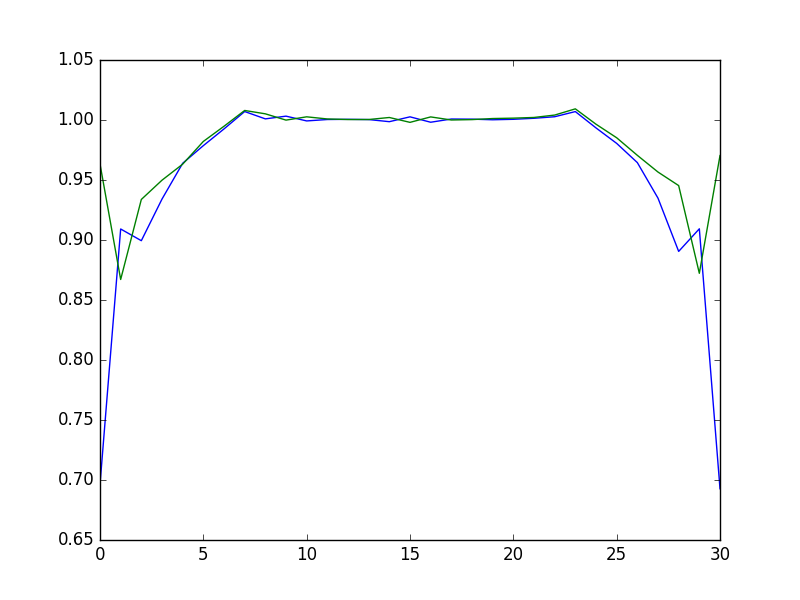
\includegraphics[width=0.8\linewidth]{reconstruction_potential.png}
    \caption{
            Плотности электронов со спином вверх и вниз в самосогласованном решении
            для топологического изолятора с точечным отталкиванием
            }
    \label{fig:rec_potential}
\end{figure}
\begin{figure}
    \centering
    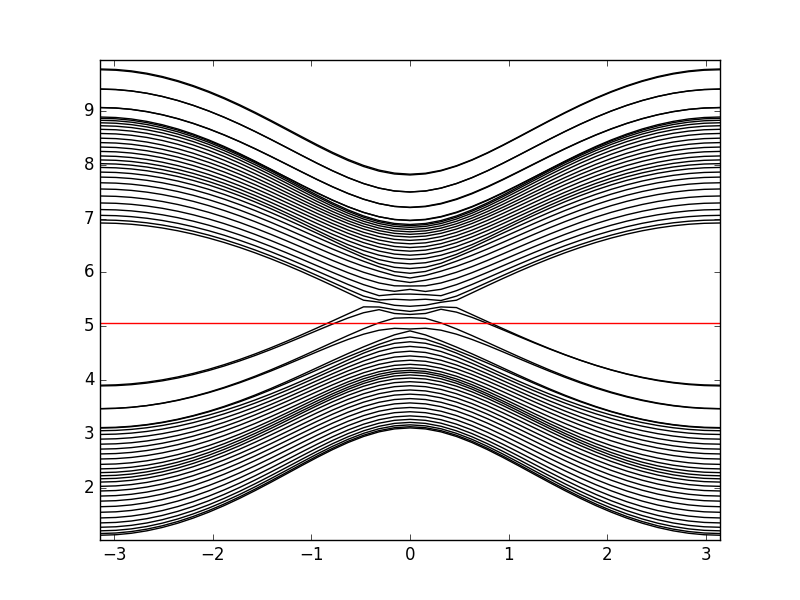
\includegraphics[width=0.8\linewidth]{reconstruction_spectrum_up.png}
    \caption{
            Спектр электронов со спином вверх в самосогласованном потенциале. Красная 
            линия означает уровень Ферми.
            }
    \label{fig:spin_up}
\end{figure}
\begin{figure}
    \centering
    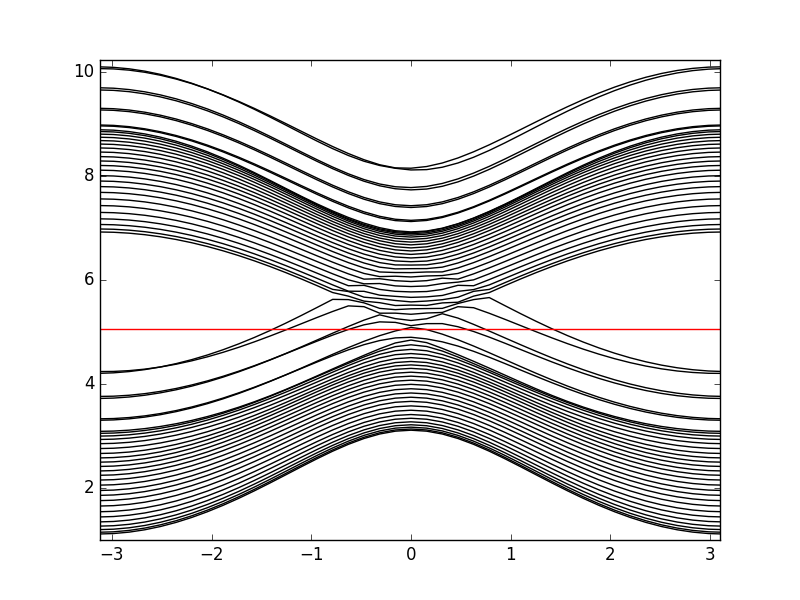
\includegraphics[width=0.8\linewidth]{reconstruction_spectrum_down.png}
    \caption{Спектр электронов со спином вниз в самосогласованном потенциале. Красная 
            линия означает уровень Ферми.}

    \label{fig:spin_down}
\end{figure}
